\documentclass{sysuthesis}

\usepackage{multicol}
\usepackage{multirow}



%%
% 论文相关信息
% 本文档中前缀"c-"代表中文版字段, 前缀"e-"代表英文版字段
% modifyer: 黄俊杰(huangjj27, 349373001dc@gmail.com)
% update date: 2017-04-13
%%

% 标题
% 论文题目应以简短、明确的词语恰当概括整个论文的核心内容,避免使用不常见的缩略词、缩写字。读者通过标题可大致了解毕业设计(论文)的内容、专业的特点和科学的范畴。中文题目一般不宜超过 24 个字,必要时可增加副标题。外文题目一般不宜超过 12 个实词

% 封面标题。由于技术所限,封面题目过长的划分交由用户您进行定夺
% 这也能让您的论文封面看起来更有美感
\covertitlefirst{蛇形机器人爬杆运动}
\covertitlesecond{的快速自适应控制}

% Author:   Souler Ou
% 修改者:    欧一锋
% Date:     3/30/2018
% Mail:     ou@souler.cc
%如果英文标题过长可以使用此两项作为表三(答辩记录表)的标题。
\etitlefirst{Unofficial \Latex\ Template}
\etitlesecond{for SYSU Graduation Thesis}

% 另外一种封面的论文题目. 换行使用换行符("\\")
%\title{
%    中山大学 \\
%    本科毕业论文非正式模版
%}

% 中文标题
\ctitle{蛇形机器人爬杆运动的快速自适应控制}
\etitle{Fast Adaptive Control Of Snake Robots For Pole Climbing}

% 解决英文摘要页标题过长问题 (Issue 49&63)
% 当\etitle的长度超过页边距时,请使用下面的命令自行断行
% 此操作只影响英文摘要页的标题,不影响页眉的标题
% 如果不需要断行,将\eabstracttitlesecond{ }留空即可
\eabstracttitlefirst{Fast Adaptive Control Of} 
\eabstracttitlesecond{Snake Robots For Pole Climbing}

% 作者详细信息
\author{简智勇}
\cauthor{简\ 智\ 勇}    % 封面作者
\eauthor{Jian Zhiyonf}
\studentid{15352146}
\cschool{数据科学与计算机学院}

\cmajor{软件工程}
\emajor{Software Engineering}

% 指导老师
\cmentor{黄凯\ 教授}
\ementor{Prof. Huang Kai}

     % 论文相关信息
%%
% 开题报告
% modifier: 黄俊杰(huangjj27, 349373001dc@gmail.com)
% update date: 2017-05-14

% 选题目的
\objective{
	\qquad 蛇形机器人是一类仿生超冗余度机器人,用于模拟蛇类生物在野生环境中的仿生运动,具有快速、稳定、多样性等特点。这些蛇形机器人多数是由许多活动关节模块连接组成,从而赋予它们运动学上的多功能性,如弯曲、伸展和盘绕。蛇形机器人已经应用在各个领域,如救灾、工厂维护和恐怖主义的监视任务。
	
	\qquad 为了更好地完成预定义的任务,蛇形机器人需要获得自主移动和自适应行为的能力,例如,根据其所处环境的不同情况决定何时、何地以及如何移动来自动适应环境,然而这种实现是并不容易的。首先,由于蛇形机器人具有冗余的自由度,使得机器人的运动建模比较困难,尤其是机器人与环境之间复杂的相互作用,使得多自由度机器人的运动控制更加复杂。第二,当遇到事先未知的环境时,显而易见的需要确定可控制的策略。即使对于给定的控制策略,如何确定其参数也不简单。第三,确定控制策略及其相应参数的运行时过程必须是有效的,即实时的。否则,机器人的期望运动将很可能失败。
	
	\qquad 为了让机器人适应未知环境,利用传感器感知环境和嵌入环境感知规则的方法已经被广泛使用。提出了一种基于CPG(中心模式发生器)模型的控制策略。提出了一种基于状态估计的蛇形机器人自适应控制。由于这些方法中的模型是基于状态估计的梯度模型。有研究者提出了结合物理环境信息的神经网络模型来确定控制方案,然而这些模型仅仅是控制建议。
	
	\qquad 所以本课题提出一种新的蛇形机器人自适应控制框架。基于离线无监督训练收集的数据,我们的框架能够通过快速回归有效地适应环境变化的新的控制参数的值。具体来说,我们的目标是爬杆,这需要快速响应环境的变化即杆的半径的变化。在这种情况下,如果机器人的运动不能做到及时适应,机器人就会掉下来。为了评价该方法的有效性,我们计划对蛇形机器人在不同杆上进行了实验以及对于不同爬杆步态采用算法进行实验。
	

}

% 思路
\methodology{
	\qquad 通过数据驱动的方式,基于蛇形机器人爬杆时所用的步态——Rolling步态,主要分成两大步骤:
	\begin{enumerate}
		\item OFFLINE训练:确认参数的变化空间,然后进行离线的训练,采集训练数据(如关节角度,参数值,速度等)。然后对采集的大量数据进行一个预处理,使用聚类方法进行归类。
		\item ONLINE算法驱动:通过实时地按照一定频率不断调用算法来调整蛇形机器人的步态参数值。通过利用回归分析来获取所需要修改的参数值来调整蛇形机器人的步态。
	\end{enumerate}
}

% 研究方法/程序/步骤
\researchProcedure{
	\qquad 本研究采用的研究方法如下:
	\begin{enumerate}
		\item 相关论文查找,归类,阅读及综合分析;
		\item 实验环境的搭建(仿真模型的建模或者实物机器人的构建和检测);
		\item 算法代码的编写实现;
		\item 进行样例实验检测算法的可行性和对比实验检测算法的有效性;
		\item 收集实验数据进行实验结果的对比分析;
	\end{enumerate}
}

% 相关支持条件
\supportment{
	\qquad 实验所需的软硬件为:
	\begin{enumerate}
		\item V-REP仿真平台;
		\item 带有Linux操作系统的主机一台;
		\item 蛇形机器人实物;
		\item 各种元件模块如wifi,芯片等;
	\end{enumerate}
}

% 进度安排
\schedule{
	\qquad 整体进度安排如下:
	\begin{itemize}
		\item 2018.12-2019.01 进行文献查阅,确认算法实现框架;
		\item 2019.01-2019.02 进行实验环境的搭建和算法代码的编写实现;
		\item 2019.02-2019.03 进行样例实验以及对比实验,采集实验数据;
		\item 2019.03-2019.04 进行实现结果分析以及学位论文初稿的撰写;
		\item 2019.04-2019.05 进行算法或者实验的优化,在指导老师的意见下对学位论文进行更进一步地修改;
		\item 2019.05-2019.06 准备毕业论文答辩;
	\end{itemize}
}

% 指导老师意见
\proposalInstructions{

}

   % 开题报告内容
%%
% 摘要信息
% 本文档中前缀"c-"代表中文版字段, 前缀"e-"代表英文版字段
% 摘要内容应概括地反映出本论文的主要内容,主要说明本论文的研究目的、内容、方法、成果和结论。要突出本论文的创造性成果或新见解,不要与引言相 混淆。语言力求精练、准确,以 300—500 字为宜。
% 在摘要的下方另起一行,注明本文的关键词(3—5 个)。关键词是供检索用的主题词条,应采用能覆盖论文主要内容的通用技术词条(参照相应的技术术语 标准)。按词条的外延层次排列(外延大的排在前面)。摘要与关键词应在同一页。
% modifier: 黄俊杰(huangjj27, 349373001dc@gmail.com)
% update date: 2017-04-15
%%

\cabstract{
蛇形机器人是由多个可活动关节进行连接,具有超高冗余度的一种仿生机器人。然而,这种机器人的自主性运动是一个十分复杂的问题。本文提出了蛇形机器人爬杆运动中的一套自适应控制框架。通过对无监督训练的数据进行聚类和多参数的快速回归,我们的控制框架能够保证蛇形机器人在爬杆运动中对环境变化做出快速反应。我们的实验结果表明了通过利用该控制框架,蛇形机器人在运动过程中选择新的控制参数进行调整的时间开销约为100ms,并且蛇形机器人可以去爬升不同直径的杆。
}
% 中文关键词(每个关键词之间用“;”分开,最后一个关键词不打标点符号。)
\ckeywords{蛇形机器人;自动化运动;爬杆运动;加权回归;机器学习}

\eabstract{
Snake-liked robots are a class of biomorphic hyper-redundant robots consist of many chain-connected active joint modules. Autonomy of this kind of robots is however a complex problem. This paper proposes an adaptive control framework for the pole climbing of snake robots. By clustering the unsupervised training data and fast multi-parameter regression, our framework can rapidly react to environment changes. Experimental results show that, by using our framework, the overhead of choosing a control parameter and setting a new value for it is about 100 ms and our snake robot can climb poles with different diameters.
}
% 英文文关键词(每个关键词之间用半角加空格分开, 最后一个关键词不打标点符号。)
\ekeywords{Snake-liked robots; autonomous ability; pole climbing; weighted regression; machine learning}

     % 摘要内容
%%
% 成绩评定记录表
% modifier: 黄俊杰(huangjj27, 349373001dc@gmail.com)
% update date: 2017-05-17

\gradingComment{
  某某同学针对什么问题研究了什么算法/实现了什么系统/针对这个系统做了什么测试,本文选题合理,实验结果表明技术路线……论文写作规范,引用文献充分,符合中山大学本科论文的规范,是篇优秀/良好/中等/合格的论文。
}
    % 成绩评定记录表评语
%%
% 四次进度报告相关信息

% Author:   Souler Ou
% 修改者:    欧一锋
% Date:     3/30/2018
% Mail:     ou@souler.cc

% 第一次进度报告
\firstsummary{
	\begin{adjustwidth}{2em}{2em}
		在这一阶段,XXX工作基本完成,主要在如下几个方面:
		\begin{enumerate}
			\item 完成了第一项。
			\item 完成了第二项
			\item 完成了第三项。 
		\end{enumerate}
	\end{adjustwidth}
}
% 第2次进度报告
\secondsummary{
	\begin{adjustwidth}{2em}{2em}
		...
	\end{adjustwidth}
}
% 第3次进度报告
\thirdsummary{
	\begin{adjustwidth}{2em}{2em}
		...
	\end{adjustwidth}
}
% 第4次进度报告
\fourthsummary{
	\begin{adjustwidth}{2em}{2em}
		...
	\end{adjustwidth}
}
% 第1次老师评价
\firstcomment{
	\begin{adjustwidth}{2em}{2em}
		论文完成情况良好。
	\end{adjustwidth}
}
% 第2次老师评价
\secondcomment{
	\begin{adjustwidth}{2em}{2em}
		...
	\end{adjustwidth}
}
% 第3次老师评价
\thirdcomment{
	\begin{adjustwidth}{2em}{2em}
		...
	\end{adjustwidth}
}
% 第4次老师评价
\fourthcomment{
	\begin{adjustwidth}{2em}{2em}
		...
	\end{adjustwidth}
}
% 老师总评价
\finalcomment{
	\begin{adjustwidth}{2em}{2em}
		...
	\end{adjustwidth}
}   % 过程检查报告数据
\begin{document}
    % 论文前置部分
    \frontmatter
        \pagenumbering{Roman}
        \maketitle    % 封面
        \makeProposal% 开题报告
        \makeProgressCheck  % 过程检查记录表
        \makeDefenseRecord  % 答辩情况等级表
        \makedisclaim       % 学术诚信声明
        \makeabstract       % 中英文摘要
        \maketableofcontents        % 目录
        \makelistoffiguretable

    % 论文主体部分
    \mainmatter
        % 引言

        % 正文
        %%
% 引言或背景
% 引言是论文正文的开端,应包括毕业论文选题的背景、目的和意义;对国内外研究现状和相关领域中已有的研究成果的简要评述;介绍本项研究工作研究设想、研究方法或实验设计、理论依据或实验基础;涉及范围和预期结果等。要求言简意赅,注意不要与摘要雷同或成为摘要的注解。
% modifier: 黄俊杰(huangjj27, 349373001dc@gmail.com)
% update date: 2017-04-15
%%

\chapter{引言}
%定义,过去的研究和现在的研究,意义,与图像分割的不同,going deeper
\label{cha:introduction}
\section{选题背景与意义}
\label{sec:background}
% What is the problem
% why is it interesting and important
% Why is it hards, why do naive approaches fails
% why hasn't it been solved before
% what are the key components of my approach and results, also include any specific limitations,do not repeat the abstract
%contribution
蛇形机器人是一类具有高冗余度的仿生机器人~\cite{Chirikjian1995The}。蛇形机器人设计核心在于模仿生物蛇的独特的无肢运动以及生物蛇在野外表现出的出色的快速,稳定,多样的运动能力和方式。仿生蛇形机器人通常是由许多可活动关节模块连接组成,这种组成方式可赋予蛇形机器人多样的运动形式,例如弯曲和伸缩,蛇形机器人的模块间结构给蛇形机器人像生物蛇一样做蜿蜒运动,侧移运动或者伸缩运动提供了结构基础。蛇形机器人已经应用在各个领域,例如灾难的救援(地震之后的救援探测),工厂管道的维护和应用于恐怖事件中作监视作用。

为了更好的完成预定义的任务,蛇形机器人需要获得自主移动和自适应环境及调整自身行为运动的能力~\cite{Liljeb2013Snake},例如,根据自身和环境的不同情况决定何时何地以及如何移动。然而,自适应环境去调整自身的运动并不是一件简单的事情。原因是多方面的。首先,高冗余的自由度给蛇形机器人的运动建模制造了很大的困难,特别是在机器人和环境之中的复杂交互中建模尤为困难。多自由度的蛇形机器人结构使其对应的控制方案更加的复杂。其次,当遇到未知的环境时,如何确定合适的控制策略显然是一个关键性的问题。即使对于一个给定的策略,如何确定控制参数的值来使得蛇形机器人能够做出期望的运动也不是可以一步到位的。第三,决定控制策略及其相应的参数必须在实时的运动过程中做到有效,迅速,即时,否则蛇形机器人的运动很有可能会失败甚至导致蛇形机器人的损坏。

本文提出了一种新的蛇形机器人的自适应控制模型。本文模型基于无监督训练离线收集经验数据,然后通过快速回归分析得到新的控制参数值来有效地适应环境的变化。具体来说,本文实验以在爬杆过程中蛇形机器人对环境变化的快速响应为目标。因为在爬杆过程中,如果控制策略不能做到及时,准确,那么机器人就会出现因为杆的直径发生变化从而从杆上掉落的情况。为了评估本文模型的有效性,本文让蛇形机器人在本文提出的控制策略控制下在不同直径的杆上进行攀爬运动。本文的意义在于:
\begin{itemize}
	\item 提出了一个蛇形机器人爬杆的自适应控制模型。 对于离线无监督训练,使用$K$均值聚类的改进版算法——$K-MEANS++$算法对收集的数据进行聚类。 在运行期间,将机器人的Z轴速度用作反馈信号,以不断调整机器人的新控制参数。
	\item 将一个多元回归模型简化成一个一元回归模型来实时计算最优的控制参数值,通过熵方差实时去选出当前状态下的最敏感控制参数。然后仅仅通过对这个参数做回归分析计算,将一个多参数回归模型转换成了一个一元回归模型。
	\item 实验结果表明,运行时的算法开销平均值略大于100\,ms并且蛇形机器人可以快速自适应在不同直径的杆上的攀爬运动,顺利在杆上做盼盼运动。
\end{itemize}

\section{国内外研究现状}
\label{sec:related_work}

为了让蛇形机器人适应未知的环境,能够在未知环境中做出正确的运动姿态,使用嵌入式传感器来感知环境并根据传感器数据做出对应的环境感知之后做出相对应的控制算法的方法已被广泛使用~\cite{BalancingAndControl}~\cite{FeedbackControlOfSoft}~\cite{CPGenabling}~\cite{GaitBasedCompliant}。唐超权等提出了一种基于多模态CPG(中枢模式发生器)模型的控制策略~\cite{CPGenabling},该控制策略是基于预定义的预期速度值,利用当前速度和预期速度的关系来自调整输入信号进而诱导CPG模型做出运动的改变的多模态CPG模型。Rollinson等提出了一种基于状态估计的蛇形机器人自适应控制方案~\cite{GaitBasedCompliant}。通过EKF(扩展卡尔曼滤波)整合传感器信息在每个时间步长处有效地估计基于步态的蛇形机器人状态,然后选择相对于该状态的参数控制空间来控制机器人的运动。 以上两种控制方案的提出在相应场景下对机器人的控制比人类去单独控制每一个控制参数来控制机器人以及固有的运动方程控制方案确实更有效,且能运用更丰富灵活的步态运动。然而参数化步态和中央模式生成器~\cite{ijspeert2008central}这样的简单控制器虽然已经取得了一些成功,但使用这些控制器创建自主或自适应行为已经证明是困难的。同时对于自适应运动我们也要考虑效率上的问题。在如今人工智能的浪潮下,对于机器人的自适应控制,有研究人员提出神经网络模型结合物理环境信息来确定控制方案~\cite{InformationDriven}~\cite{NovelPlasticityRule}~\cite{MissileSystems}~\cite{NeuroFuzzyBayesian},但是目前还无法通过具体实际的实验来验证。


\section{本文的论文结构与章节安排}

\label{sec:arrangement}
本文共分为五章,各章节内容安排如下:

第一章:引言,本章介绍了蛇形机器人在自适应运动控制方面的研究背景,意义,研究现状及相关工作。

第二章:蛇形机器人结构和控制方法,介绍了本文中采用的蛇形机器人设计结构以及基于正交结构设计的蛇形机器人常用控制函数。

第三章:研究方法介绍,详细地介绍了本文所采用的研究算法,介绍了算法的框架以及每个步骤的详细分析。

第四章:实验和结果展示,展示了本文所采用的算法在蛇形机器人爬杆运动中的表现情况,包括数据分析,对照实验,算法性能分析。

第五章:总结与展望。总结本文的研究结论,同时根据目前理论和实验的不足之处,对下一步的研究工作做展望。


        \newclearpage
        %\chapter{蛇形机器人结构和控制方法}
\label{cha:example}
%\section{图像的插入}
%\subsection{镶嵌在文中的图像}
%\label{sec:Images}
%\begin{wrapfigure}{r}{0.5\linewidth}
%	\centering
%	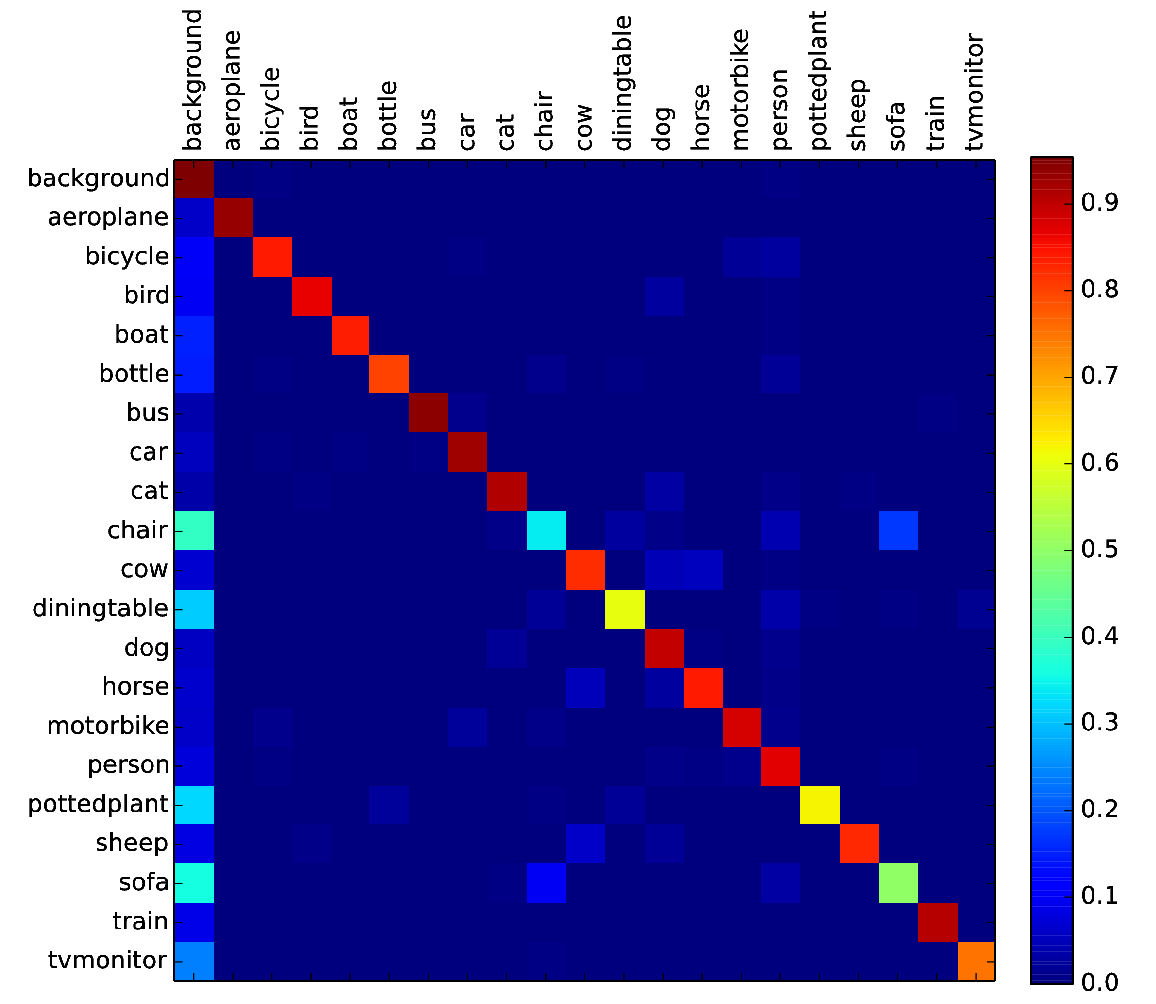
\includegraphics[width=0.5\textwidth]{image/result/confusion.pdf}
%	\caption{镶嵌在文中的图像}
%	\label{fig:confusion}
%\end{wrapfigure}
%论文主体是毕业论文的主要部分,必须言之成理,论据可靠,严格遵循本学科国际通行的学术规范。在写作上要注意结构合理、层次分明、重点突出,章节标题、公式图表符号必须规范统一。论文主体的内容根据不同学科有不同的特点,一般应包括以下几个方面: (1)毕业论文(设计)总体方案或选题的论证; (2)毕业论文(设计)各部分的设计实现,包括实验数据的获取、数据可行性及有效性的处理与分析、各部分的设计计算等; (3)对研究内容及成果的客观阐述,包括理论依据、创新见解、创造性成果及其改进与实际应用价值等; (4)论文主体的所有数据必须真实可靠,凡引用他人观点、方案、资料、数据等,无论曾否发表,无论是纸质或电子版,均应详加注释。自然科学论文应推理正确、结论清晰;人文和社会学科的论文应把握论点正确、论证充分、论据可靠,恰当运用系统分析和比较研究的方法进行模型或方案设计,注重实证研究和案例分析,根据分析结果提出建议和改进措施等。
%\subsection{单张图像的插入}
%\begin{figure}[h]
	\centering
	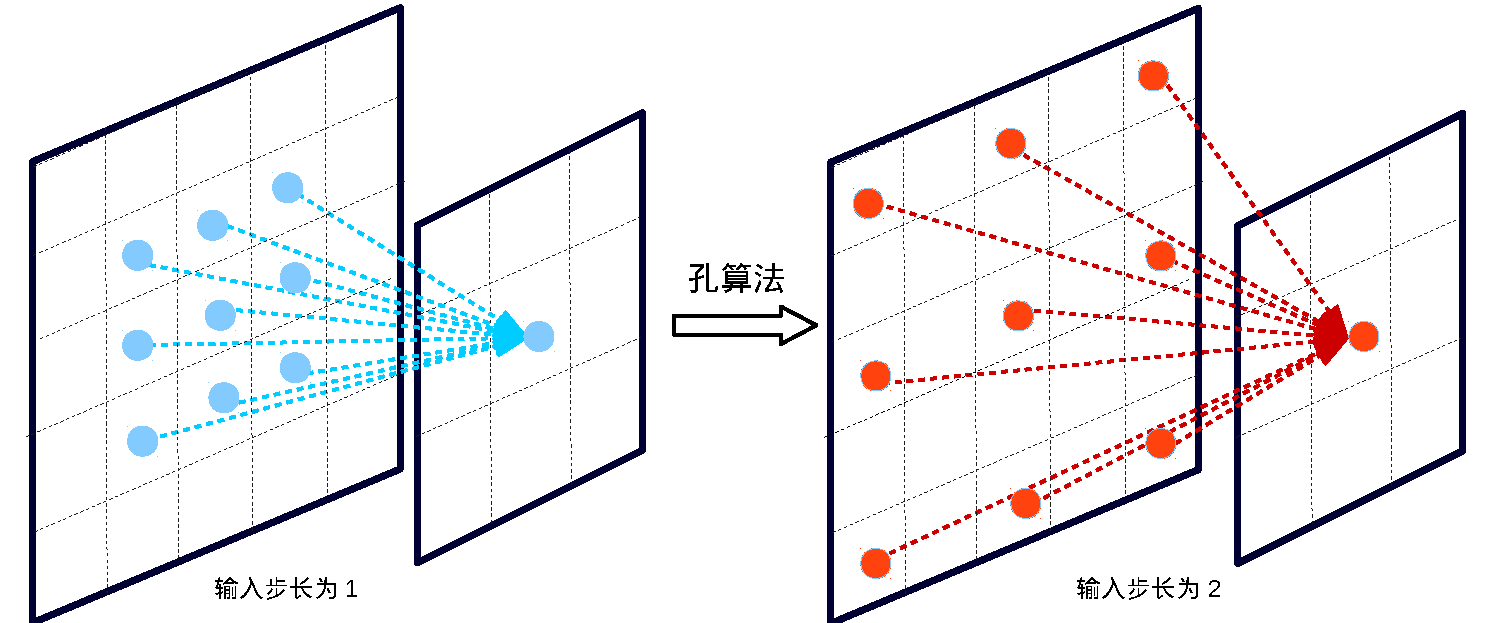
\includegraphics[width=0.5\textwidth]{image/illustration/hole.pdf}
	\caption{单张图像}
 	\label{fig:hole}
\end{figure}

%
%\subsection{多张图像的并排插入}
%\label{sub:多张图像的并排插入}
%\begin{figure}[h!]%文中的Grid-LSTM模型做的语义图像分割的例子
	\centering
	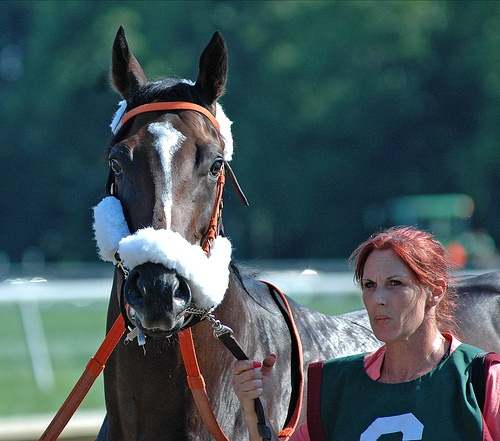
\includegraphics[width=.2\textwidth,height=.15\textwidth]{image/example/2007_000799.jpg}
	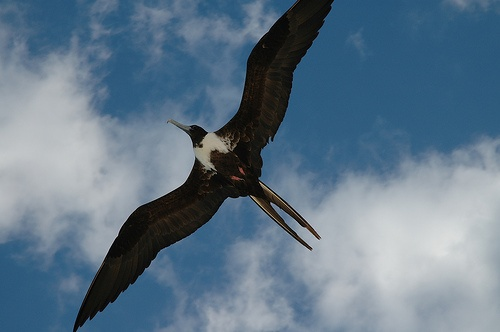
\includegraphics[width=.2\textwidth,height=.15\textwidth]{image/example/2007_002094.jpg}
	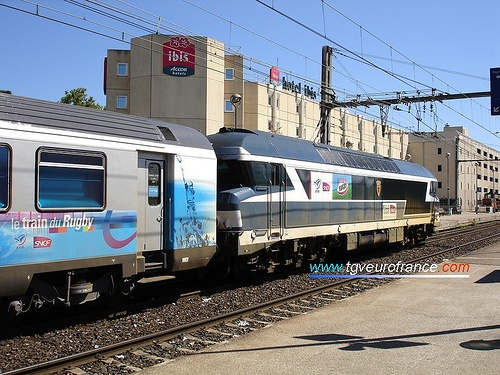
\includegraphics[width=.2\textwidth,height=.15\textwidth]{image/example/2007_004483.jpg}
	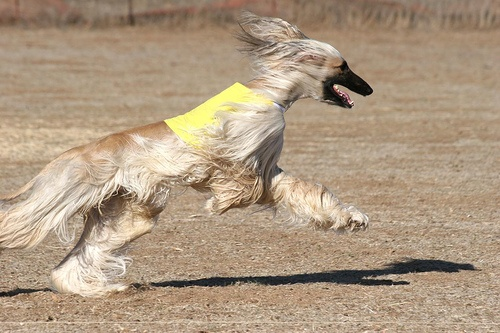
\includegraphics[width=.2\textwidth,height=.15\textwidth]{image/example/2007_003194.jpg}
	\\
	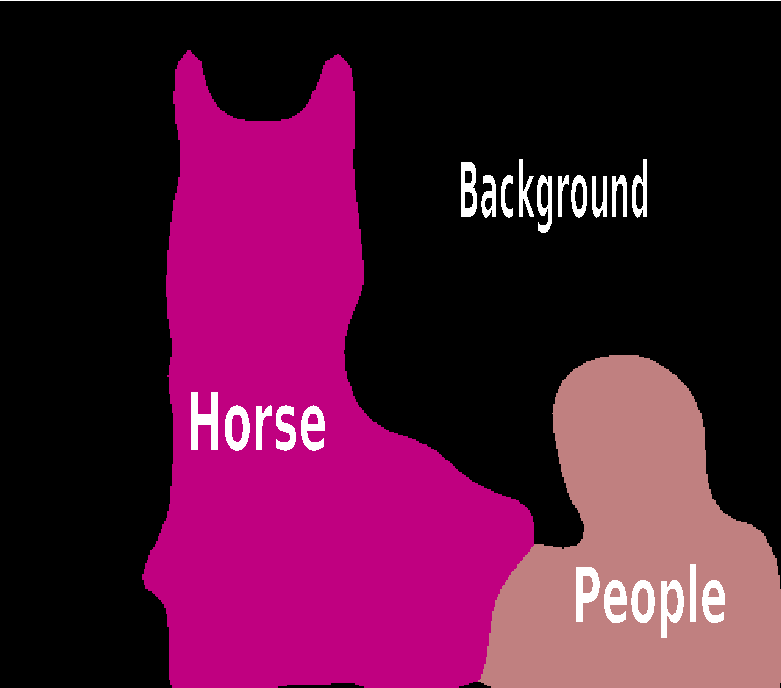
\includegraphics[width=.2\textwidth,height=.15\textwidth]{image/example/2007_000799.pdf}
	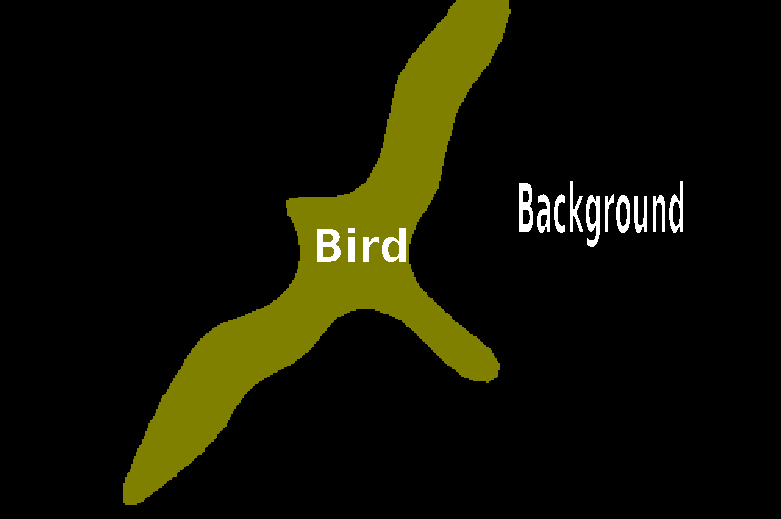
\includegraphics[width=.2\textwidth,height=.15\textwidth]{image/example/2007_002094.pdf}
	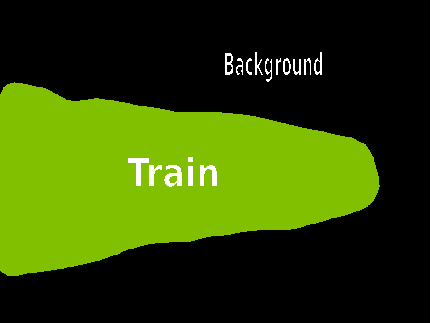
\includegraphics[width=.2\textwidth,height=.15\textwidth]{image/example/2007_004483.pdf}
	
\includegraphics[width=.2\textwidth,height=.15\textwidth]{image/example/2007_003194.pdf}
	\caption{并排的多张图像}
	\label{fig:example1}
\end{figure}
\endinput

%\begin{figure}[h]
\centering
	\makebox[0.11\textwidth]{\scriptsize 图像}
	\enspace
	\makebox[0.11\textwidth]{\scriptsize 真值}
	\enspace
	\makebox[0.11\textwidth]{\scriptsize CNN+5LSTM\textbf{1}}
	\enspace\thinspace
	\makebox[0.11\textwidth]{\scriptsize CNN+5LSTM\textbf{2}}
	\enspace\thinspace
	\makebox[0.11\textwidth]{\scriptsize CNN+5LSTM\textbf{3}}
	\enspace\thinspace
	\makebox[0.11\textwidth]{\scriptsize CNN+5LSTM\textbf{4}}
	\enspace\thinspace
	\makebox[0.11\textwidth]{\scriptsize CNN+5LSTM\textbf{5}}\\
	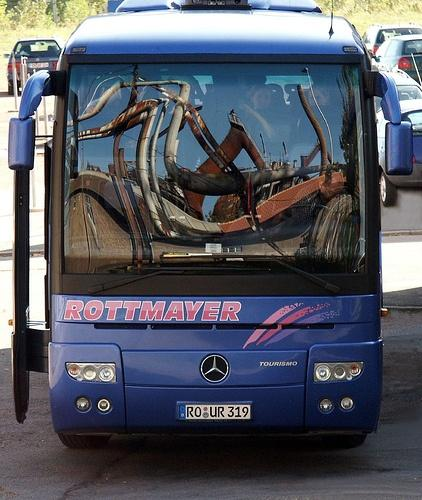
\includegraphics[width=0.11\textwidth]{image/improvement/2007_000663.jpg}
	\enspace\thinspace %\hfill
	
\includegraphics[width=0.11\textwidth]{image/improvement/2007_000663.png}
	\enspace\thinspace
	
\includegraphics[width=0.11\textwidth]{image/improvement/2007_000663_1.png}
	\enspace\thinspace
	
\includegraphics[width=0.11\textwidth]{image/improvement/2007_000663_2.png}
	\enspace\thinspace
	
\includegraphics[width=0.11\textwidth]{image/improvement/2007_000663_3.png}
	\enspace\thinspace
	
\includegraphics[width=0.11\textwidth]{image/improvement/2007_000663_4.png}
	\enspace\thinspace
	
\includegraphics[width=0.11\textwidth]{image/improvement/2007_000663_5.png}
	\enspace\thinspace
	\caption{并排的多张图像加各自的注解}
	\label{fig:improvement}
\end{figure}

%
%\subsection{两列图像的插入}
%\label{sec:complex}
%\begin{figure}[h!] % image examples & compare
	\begin{subfigure}{0.55\textwidth}
		\makebox[0.18\textwidth]{\scriptsize Grid-5LSTM}
		\makebox[0.18\textwidth]{\scriptsize FCN-8s\cite{long2015fully}}
		\makebox[0.18\textwidth]{\scriptsize SDS\cite{hariharan2014simultaneous}}
		\makebox[0.18\textwidth]{\scriptsize 真值}
		\makebox[0.18\textwidth]{\scriptsize 图像} \\
		
\includegraphics[width=0.18\textwidth]{image/result/compare/my_horse.pdf}
		
\includegraphics[width=0.18\textwidth]{image/result/compare/fcn_horse.png}
		
\includegraphics[width=0.18\textwidth]{image/result/compare/sds_horse.png}
		
\includegraphics[width=0.18\textwidth]{image/result/compare/gt_horse.pdf}
		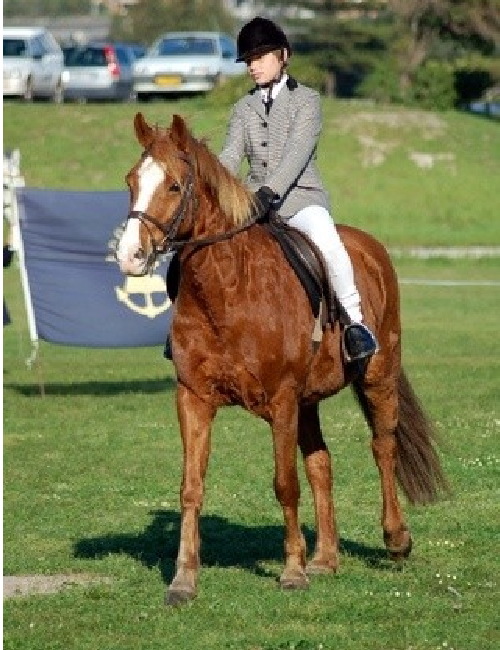
\includegraphics[width=0.18\textwidth]{image/result/compare/im_horse.pdf}
		\\
		
\includegraphics[width=0.18\textwidth]{image/result/compare/my_motor.png}
		
\includegraphics[width=0.18\textwidth]{image/result/compare/fcn_motor.png}
		
\includegraphics[width=0.18\textwidth]{image/result/compare/sds_motor.png}
		
\includegraphics[width=0.18\textwidth]{image/result/compare/2007_005173.png}
		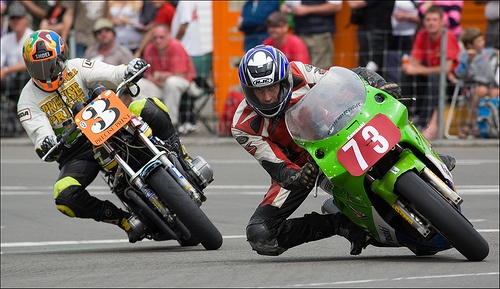
\includegraphics[width=0.18\textwidth]{image/result/compare/2007_005173.jpg}
		\\
		
\includegraphics[width=0.18\textwidth]{image/result/compare/my_sheep.pdf}
		
\includegraphics[width=0.18\textwidth]{image/result/compare/fcn_sheep.png}
		
\includegraphics[width=0.18\textwidth]{image/result/compare/sds_sheep.png}
		
\includegraphics[width=0.18\textwidth]{image/result/compare/gt_sheep.pdf}
		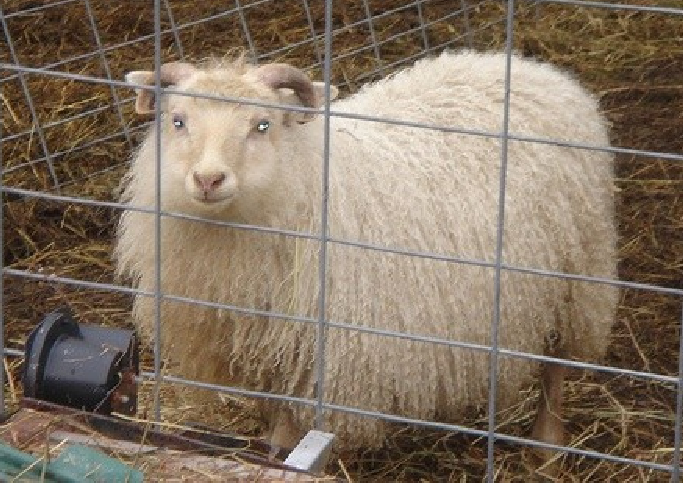
\includegraphics[width=0.18\textwidth]{image/result/compare/im_sheep.pdf}
		\\
		
\includegraphics[width=0.18\textwidth]{image/result/compare/my_boat.png}
		
\includegraphics[width=0.18\textwidth]{image/result/compare/fcn_boat.png}
		
\includegraphics[width=0.18\textwidth]{image/result/compare/sds_boat.png}
		
\includegraphics[width=0.18\textwidth]{image/result/compare/2007_004241.png}
		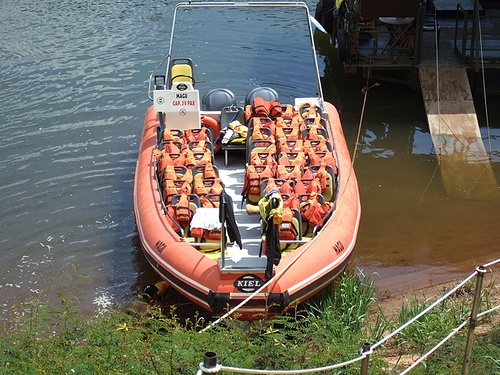
\includegraphics[width=0.18\textwidth]{image/result/compare/2007_004241.jpg}
		\caption{左边的图像}
		\label{fig:compare1}
	\end{subfigure}
	\begin{subfigure}{0.4\textwidth}
		\centering
%		\makebox[0.3\textwidth]{} \\
%		\makebox[0.3\textwidth]{} \\
		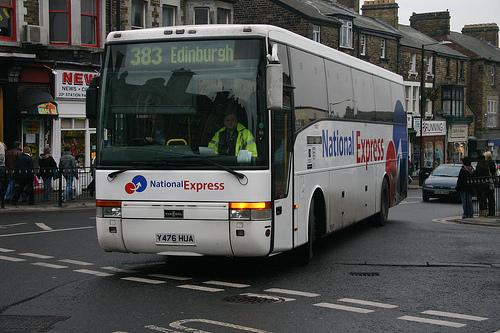
\includegraphics[width=0.25\textwidth]{image/result/compare/2010_005284.jpg}
		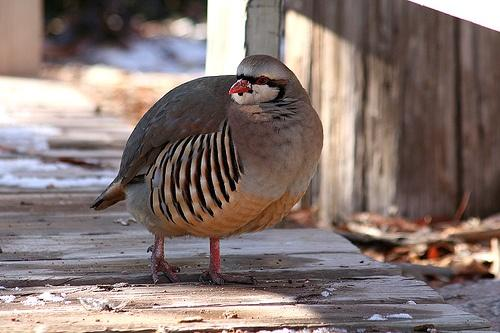
\includegraphics[width=0.25\textwidth]{image/result/compare/2007_003349.jpg}
		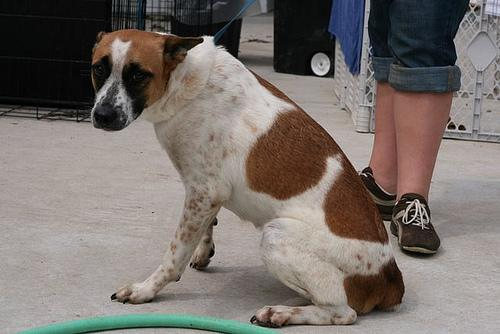
\includegraphics[width=0.25\textwidth]{image/result/compare/2009_004507.jpg} 
		\\
		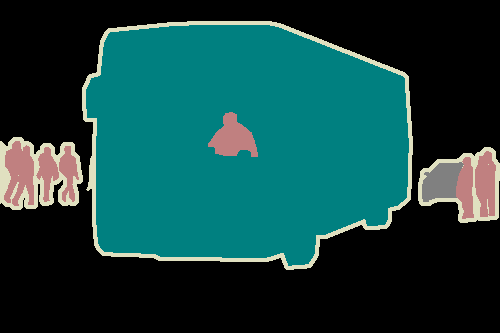
\includegraphics[width=0.25\textwidth]{image/result/compare/2010_005284.png}
		
\includegraphics[width=0.25\textwidth]{image/result/compare/2007_003349.png}
		
\includegraphics[width=0.25\textwidth]{image/result/compare/2009_004507.png} \\
		
\includegraphics[width=0.25\textwidth]{image/result/compare/zoom_bus.png}
		
\includegraphics[width=0.25\textwidth]{image/result/compare/zoom_bird.png}
		
\includegraphics[width=0.25\textwidth]{image/result/compare/zoom_dog.png} \\
		
\includegraphics[width=0.25\textwidth]{image/result/compare/deeplab_bus.png}
		
\includegraphics[width=0.25\textwidth]{image/result/compare/deeplab_bird.png}
		
\includegraphics[width=0.25\textwidth]{image/result/compare/deeplab_dog.png} \\
		
\includegraphics[width=0.25\textwidth]{image/result/compare/my_bus.png}
		\includegraphics[width=0.25\textwidth]{image/result/compare/my_bird.png}
		\includegraphics[width=0.25\textwidth]{image/result/compare/my_dog.png} 
		\caption{右边的图像}
		\label{fig:compare2}
	\end{subfigure}
	\caption{复杂的两列对象的插入}
	\label{fig:complex}
\end{figure}

%
%\clearpage
%
%\section{表格的插入}
%\label{sec:tables}
%\begin{table}[h] %voc table result
	\centering
		\begin{tabular}{*{4}{c}}
			\toprule
	 		Method & Pixel Acc. & Mean Acc. & Mean Iu.\\
			\midrule
			Liu等人\cite{liu2011sift}  & 76.7 & - & -\\
		Tighe等人\cite{tighe2013finding}  & 78.6 & 39.2 & -\\
			FCN-16s\cite{long2015fully} & 85.2 & \textbf{51.7} & 39.5\\
			Deeplab-LargeFOV\cite{chen14semantic} & 85.6 & 51.2 & 39.7\\
			\midrule
			Grid-LSTM5 & \textbf{86.2} & 51.0 & \textbf{41.2}\\
			\bottomrule
		\end{tabular}
		\caption{典型的实验对比表格}		
		\label{tab:siftflow}
\end{table}

%\begin{table}[h] %voc table result
\centering
	\resizebox{\textwidth}{!}{
	\begin{tabular}{c|*{20}{c}|c}
		\toprule
		Method & aero & bike & bird & boat & bottle & bus & car & cat & chair & cow & table & dog & horse & mbike & person & plant & shep & sofa & train & tv & mIoU.\\
		\midrule
		CNN				   & 72.6 & 29.6 & 70.2 & 53.1 & 65.1 & 81.0 & 74.3 & 79.8 & 25.0 & 64.8 & 47.8 & 69.5 & 66.2 & 65.2 & 74.2 & 42.1 & 69.6 & 38.8 & 74.4 & 58.6 & 62.5\\
		CNN+\textbf{1}LSTM & 71.5 & 30.6 & 70.5 & 53.8 & 64.9 & 82.4 & 77.1 & 79.5 & 25.1 & 65.8 & 47.8 & 71.5 & 64.6 & 67.0 & 74.0 & 43.9 & 69.6 & 38.6 & 74.9 & 59.4 & 63.0\\
		CNN+\textbf{2}LSTM & 76.1 & 32.6 & 72.1 & 57.0 & 65.3 & 83.6 & 75.4 & 81.7 & 24.7 & 69.3 & 47.5 & 72.3 & 68.9 & 69.5 & 74.7 & 41.5 & 69.8 & 38.3 & 77.8 & 62.1 & 64.3 \\
		CNN+\textbf{3}LSTM & 77.7 & 32.3 & 72.6 & 60.0 & 68.3 & 85.5 & 78.5 & 82.3 & 25.3 & 71.1 & 49.7 & 71.5 & 69.7 & 70.8 & 75.9 & 47.9 & 71.2 & 38.9 & 80.2 & 61.7 & 65.8 \\
		CNN+\textbf{4}LSTM & 79.1 & \textbf{33.7} & \textbf{73.6} & \textbf{62.0} & \textbf{70.4} & 85.5 & \textbf{80.9} & 83.7 & \textbf{24.1} & 70.7 & 45.7 & 73.7 & 69.6 & 72.1 & 75.6 & 47.2 & \textbf{76.0} & 37.3 & 80.5 & 62.2 & 66.4 \\
		CNN+\textbf{5}LSTM & \textbf{79.9} & 33.6 & \textbf{73.6} & 61.7 & 68.0 & \textbf{88.5} & \textbf{80.9} & \textbf{84.0} & 23.6 & \textbf{71.3} & \textbf{49.7} & \textbf{73.1} & \textbf{71.3} & \textbf{72.9} & \textbf{76.4} & \textbf{48.9} & 75.1 & \textbf{38.1} & \textbf{84.5} & \textbf{63.8} & \textbf{67.2} \\
		\midrule
		CNN+\textbf{5}LSTM$^\dag$ & 84.8 & 36.4 & 82.0 & 69.4 & 73.0 & 87.2 & 81.8 & 86.1 & 34.5 & 82.4 & 53.1 & 81.5 & 77.4 & 79.0 & 81.3 & 54.8 & 81.1 & 47.0 & 84.3 & 67.3 & 72.3 \\
		\bottomrule
	\end{tabular}}
	\caption{复杂一些的表格}		
	\label{tab:vocval}
\end{table}

%
%\section{公式}
%\label{sec:formula}
%没有编号的公式
%\begin{align*}
%\begin{split}
%	\label{eq:feedforward}
%	\mybold{z}^{(l)} & = \mybold{W}^{(l)}\mybold{a}^{(l-1)} + \mybold{b}^{(l)} \\
%	\mybold{a}^{(l)} & = f(\mybold{z}^{(l)})
%\end{split}
%\end{align*}
%公式中含有中文
%\begin{align}
%	\begin{split}
%	\mbox{像素准确率} &= \sum_{i=1}^{n_{cl}}n_{ii} / \sum_{i=1}^{n_{cl}}t_i \\
%		\mbox{平均像素准确率} &= \frac{1}{n_{cl}} \sum_{i=1}^{n_{cl}}(n_{ii}/ t_i) \\
%	\mbox{Mean IU} &= \frac{1}{n_{cl}} \sum_{i=1}^{n_{cl}}\frac{n_{ii}}{t_i + \sum_j^{n_{cl}} n_{ji} - n_{ii}}
%	\end{split}
%\end{align}
%公式中含有矩阵
%\begin{equation}
%	\textbf{H} = \begin{bmatrix}
%		I*\mybold{x}_i \\ \textbf{h}
%	\end{bmatrix}
%\end{equation}
%每行后面都有编号的公式
%\begin{align}
%	\frac{\partial}{\partial W_{ij}^{(l)}} J(\mybold{W},\mybold{b};\mybold{x},y) &= \frac{\partial J(\mybold{W},\mybold{b};\mybold{x},y)}{\partial z_i^{(l+1)}}\cdot \frac{\partial z_i^{(l+1)}}{\partial W_{ij}^{(l)}} = \delta_i^{(l+1)}a_j^{(l)} \\
%	\frac{\partial}{\partial b_i^{(l)}} J(\mybold{W},\mybold{b};\mybold{x},y) &= \frac{\partial J(\mybold{W},\mybold{b};\mybold{x},y)}{\partial z_i^{(l+1)}}\cdot \frac{\partial z_i^{(l+1)}}{\partial b_i^{(l)}} = \delta_i^{(l+1)}
%\end{align}
%
%\section{算法流程图}
%\label{sec:algorithm}
%\begin{algorithm}[h]
%\KwIn{$m$个训练样本}
%\lFor{$l=1$ \emph{\KwTo} $n_l$}{
%初始化:$\Delta \mybold{W}^{(l)}=0$,$\Delta \mybold{b}^{(l)}=0$}
%\ForEach{训练样本}{
%	\lFor{$l=1$ \emph{\KwTo} $n_l-1$}{
%	前向传播:$\mybold{z}^{(l+1)}=\mybold{W}^la^l+\mybold{b}^l$,$\mybold{a}^{(l+1)}=f(\mybold{z}^{(l+1)})$}
%	输出误差计算:$\delta^{(n_l)} = \frac{\partial}{\partial \mybold{z}^{(n_l)}} J(\mybold{W},\mybold{b};\mybold{x},y)$\;
%	\lFor{$l=n_l-1$ \emph{\KwTo} $1$}{
%	后向传播:$\delta^{(l)} = \bigl((\mybold{W}^{(l)})^T \delta^{(l+1)}\bigr)f'(\mybold{z}^{(l)})$}
%	\ForAll{层l}{
%		计算梯度:$\nabla_{\mybold{W}^{(l)}}J(\mybold{W},\mybold{b};\mybold{x},y)=\delta^{(l+1)}(\mybold{a}^{(l)})^T$ \\
%		\hspace{60pt}$\nabla_{\mybold{b}^{(l)}}J(\mybold{W},\mybold{b};\mybold{x},y)=\delta^{(l+1)}$\;
%		累加梯度:$\Delta \mybold{W}^{(l)} \leftarrow \Delta \mybold{W}^{(l)} + \nabla_{\mybold{W}^{(l)}}J(\mybold{W},\mybold{b};\mybold{x},y)$; \\
%		\hspace{60pt}$\Delta \mybold{b}^{(l)} \leftarrow \Delta \mybold{b}^{(l)} + \nabla_{\mybold{b}^{(l)}}J(\mybold{W},\mybold{b};\mybold{x},y)$\;
%	}
%}
%\ForAll{层$l$}{
%	更新权重:$\mybold{W}^{(l)} \leftarrow \mybold{W}^{(l)} - \alpha \biggl[\frac 1m \Delta \mybold{W}^{(l)}]$ \\
%	\hspace{60pt} $\mybold{b}^{(l)} \leftarrow \mybold{b}^{(l)} - \alpha \biggl[\frac 1m \Delta \mybold{b}^{(l)}\biggr]$
%}
%\caption{梯度下降算法}
%\label{algo:sgd}
%\end{algorithm}
%
%\section{例子与证明}
%\subsection{例子}
%\begin{eg}
%  这是一个例子, 用以验证特殊环境的字体成功更改为楷体.
%\end{eg}
%
%\begin{proof}
%  1. 大前提
%  2. 小前提
%  结论: 示例结论
%\end{proof}
%
%\section{其他的一些用法}
%\label{sec:font}
%\subsection{子章节编号}
%\label{sec:font:subsection}
%\subsubsection{更小的章节}
%\label{sec:font:subsection:subsub}
%更小的章节编号也是支持的。
%
%\subsection{列表的使用}
%\label{src:font:list}
%
%这是一个无序列表
%\begin{itemize}
%	\item 引用文献\cite{long2015fully}
%	\item 字体{\color{red}{变红}},\textbf{粗体}
%\end{itemize}
%
%这是一个有序列表
%\begin{enumerate}
%	\item 索引前面的章节 \ref{sec:formula}、图像\ref{fig:complex}、表格\ref{tab:siftflow}
%	\item 加脚注\footnote{http://cs231n.github.io/transfer-learning/}
%\end{enumerate}
\section{蛇形机器人结构}
为了实现蛇形机器人的三维空间中的运动,Shigeo Hiorse教授的科研团队研发的ARM-R3 蛇形机器人关节间采用正交的方式相连接~\cite{Prautsch1999Control}。采用关节正交连接设计的蛇形机器人单元模块和转动副连接,最小的系统模型为三连杆模型,相邻的转动副呈现垂直的关系。最小系统模型对的关节连接模型如图\ref{fig:connect}所示,工作空间如图\ref{fig:space}所示。
\begin{figure}[h!] % image examples & compare
	\begin{subfigure}{0.5\textwidth}
		\centering
		\includegraphics[width=0.35\textwidth,height=0.15\textheight]{figure/chap03/struct.eps}
		\caption{关节连接}
		\label{fig:connect}
	\end{subfigure}
	\begin{subfigure}{0.5\textwidth}
		\centering
		\includegraphics[width=0.9\textwidth,height=0.15\textheight]{figure/chap03/space.eps}
		\caption{工作空间}
		\label{fig:space}
	\end{subfigure}
	\caption{蛇形机器人正交连接结构}
	\label{fig:Orthogonal}
\end{figure}
根据正交连接设计的蛇形机器人的实物和仿真下的建模如图\ref{fig:snakeexample}所示。
\begin{figure}[h!] % image examples & compare
	\begin{subfigure}{0.5\textwidth}
		\centering
		\includegraphics[width=0.7\textwidth,height=0.15\textheight]{figure/chap03/realSnake.eps}
		\caption{实物蛇形机器人}
		\label{fig:realSnake}
	\end{subfigure}
	\begin{subfigure}{0.5\textwidth}
		\centering
		\includegraphics[width=0.7\textwidth,height=0.15\textheight]{figure/chap03/simulateSnake.eps}
		\caption{仿真蛇形机器人}
		\label{fig:simulateSnake}
	\end{subfigure}
	\caption{蛇形机器人正交连接设计示例}
	\label{fig:snakeexample}
\end{figure}

\section{蛇形机器人步态方程}
%\begin{wrapfigure}{r}{0.4\linewidth}
%	\centering
%	\includegraphics[width=0.2\textwidth]{figure/chap03/poleclimb.eps}
%	\caption{爬杆运动}
%	\label{fig:poleclimb}
%\end{wrapfigure}
如今广泛被使用的一个蛇形机器人控制策略是基于Hirose教授提出的正弦运动模型~\cite{HiroseSine}。之后Tesch教授提出了一个蛇形机器人基于正弦运动模型的三维运动参数方程~\cite{ChosetSine}。该参数方程简化了蛇形机器人的控制策略,并实现了用少量控制参数来确定机器人的运动模型。我们实验中采用的是滚动步态~\cite{Enner2013Motion}作为实验中的爬杆步态。滚动步态的正弦运动模型函数如算式\ref{basicRoll}所示:
\begin{eqnarray}\label{basicRoll}
T_i=\left\{
\begin{array}{lr}
A\cdot \sin (\omega \cdot t + i\cdot \varepsilon )&odd\\
A\cdot \sin (\omega \cdot t + i\cdot \varepsilon +  \frac{\pi}{2})&even
\end{array}
\right.
\end{eqnarray}
\begin{figure}[h!] % image examples & compare
	\begin{subfigure}{0.5\textwidth}
		\centering
		\includegraphics[width=0.5\textwidth]{figure/chap03/pipecrawl.eps}
		\caption{管内攀爬}
		\label{fig:pipecrawl}
	\end{subfigure}
	\begin{subfigure}{0.5\textwidth}
		\centering
		\includegraphics[width=0.5\textwidth]{figure/chap03/poleclimb.eps}
		\caption{管外攀爬}
		\label{fig:poleclimb}
	\end{subfigure}
	\caption{蛇形机器人滚动步态的管道内外攀爬运动}
	\label{fig:polecc}
\end{figure}

通过修改算式\ref{basicRoll}中的幅度参数$A$,相位参数$\varepsilon$和角速度参数$\omega$, 关节的最大可转动角度,机器人的螺旋化程度,蛇形机器人的运动速率会对应地发生改变。与生物蛇不同的是蛇形机器人可以表现出生物蛇无法表现的滚动步态。虽然滚动步态很简单,但是滚动步态确是十分有效的一种运动方式(图\ref{fig:poleclimb})。 通过给予合适的参数,蛇形机器人可以通过滚动步态在地上或者管道内外等环境进行运动。

        %\newclearpage
        \chapter{研究方法}
\label{cha:method}

\section{蛇形机器人结构}


\section{蛇形机器人步态方程}
%\begin{wrapfigure}{r}{0.4\linewidth}
%	\centering
%	\includegraphics[width=0.2\textwidth]{figure/chap03/poleclimb.eps}
%	\caption{爬杆运动}
%	\label{fig:poleclimb}
%\end{wrapfigure}
如今广泛被使用的一个蛇形机器人控制策略是基于Hirose教授提出的正弦运动模型~\cite{HiroseSine}。之后Tesch教授提出了一个蛇形机器人基于正弦运动模型的三维运动参数方程~\cite{ChosetSine}。该参数方程简化了蛇形机器人的控制策略,并实现了用少量控制参数来确定机器人的运动模型。我们实验中采用的是滚动步态~\cite{Enner2013Motion}作为实验中的爬杆步态。滚动步态的正弦运动模型函数如算式\ref{basicRoll}所示:
\begin{eqnarray}\label{basicRoll}
T_i=\left\{
\begin{array}{lr}
A\cdot \sin (\omega \cdot t + i\cdot \varepsilon )&odd\\
A\cdot \sin (\omega \cdot t + i\cdot \varepsilon +  \frac{\pi}{2})&even
\end{array}
\right.
\end{eqnarray}
\begin{figure}[h!] % image examples & compare
	\begin{subfigure}{0.5\textwidth}
		\centering
		\includegraphics[width=0.5\textwidth]{figure/chap03/pipecrawl.eps}
		\caption{管内攀爬}
		\label{fig:pipecrawl}
	\end{subfigure}
	\begin{subfigure}{0.5\textwidth}
		\centering
		\includegraphics[width=0.5\textwidth]{figure/chap03/poleclimb.eps}
		\caption{管外攀爬}
		\label{fig:poleclimb}
	\end{subfigure}
	\caption{蛇形机器人滚动步态的管道内外攀爬运动}
	\label{fig:polecc}
\end{figure}

通过修改算式\ref{basicRoll}中的幅度参数$A$,相位参数$\varepsilon$和角速度参数$\omega$, 关节的最大可转动角度,机器人的螺旋化程度,蛇形机器人的运动速率会对应地发生改变。与生物蛇不同的是蛇形机器人可以表现出生物蛇无法表现的滚动步态。虽然滚动步态很简单,但是滚动步态确是十分有效的一种运动方式(图\ref{fig:poleclimb})。 通过给予合适的参数,蛇形机器人可以通过滚动步态在地上或者管道内外等环境进行运动。

\section{研究方法概述}
本文提出的研究方法框架如所示。 我们将研究方法分为两个主要部分:离线工作算法和运行时工作算法。
%\begin{wrapfigure}{r}{1.0\linewidth}
%	\centering
%	\includegraphics[width=0.8\textwidth]{figure/chap03/step.eps}
%	\caption{研究方法概述}
%	\label{fig:stepMap}
%\end{wrapfigure}
\begin{figure}[h]
	\centering
	\includegraphics[width=0.8\textwidth]{figure/chap03/step.eps}
	\caption{研究方法概述}
	\label{fig:stepMap}
\end{figure}

在离线工作算法中,第一步,我们先定义控制参数的变化空间,让机器人在不同的参数组合的控制方程下爬杆,在爬杆过程中控制方程中的参数是不变的。当机器人爬杆时,以2秒为周期记录机器人的速度以及关节角度。之后,将所有参数组合下爬杆采集到的数据整合在一起,对整个数据使用K-MEANS++进行聚类操作~\cite{Cluseter_ICT}~\cite{KmeansAndDeepLearning}。

在运行时工作算法中,给定机器人已初始化好的控制参数,在机器人爬杆过程中,也是以2秒为周期收集机器人实时的关节角度,速度和当前控制参数的数据值,然后通过归簇操作在离线工作算法中得到的数据簇中抽取同簇的数据集合。在获取到同簇的数据集合后,通过熵方差计算衡量每个控制参数对机器人运动的影响程度,最终挑取影响程度最大的控制参数,称为最敏感控制参数。最终通过加权回归得到最敏感控制参数需要修改的新值。

\section{离线工作算法}
在离线工作算法的预处理工作中,我们让机器人分别在直径为25\,cm 和 35\,cm的杆上进行大量的尝试性攀爬运动,并且在攀爬过程中收集存储数据,存储数据类型如表\,\ref{dataTable}所示。

\begin{table}[h]
	\begin{center}
		\caption{机器人训练时记录的数据类型}
		\label{dataTable}
		\begin{tabular}{cl cl} 
			\toprule
			\multicolumn{1}{m{3cm}}{\centering 数据类型}
			&\multicolumn{1}{m{4cm}}
			{\centering Definition}\\
			\midrule
			\multirow{2}{*}{$\theta_{m,i}$} & \multirow{2}{*}{第i个关节的关节角度值} \\
			\multirow{2}{*}{$M$} & \multirow{2}{*}{所测量的所有关节角角度的均值} \\
			\multirow{2}{*}{$\upsilon_{z}$} & \multirow{2}{*}{Z轴的速度值} \\\\	\hline
			\multirow{2}{*}{$A$} & \multirow{2}{*}{幅度(控制参数)的值} \\
			\multirow{2}{*}{$\omega$} & \multirow{2}{*}{角速度(控制参数)的值} \\
			\multirow{2}{*}{$\varepsilon$} & \multirow{2}{*}{相位(控制参数)的值} \\\\
			\bottomrule
		\end{tabular}
	\end{center}
\end{table}

我们定义$M=$$\frac{\sum_{i=1}^{n}\theta_{m,i}}{n}$其中,n是关节总数量。$\theta_{m}=\begin{bmatrix}\theta_{m,1} & \theta_{m,2} & \cdots & \theta_{m,n}\end{bmatrix}$是测量得到的关节角度值集合。控制参数矢量为$\begin{bmatrix}A& \omega&\varepsilon\end{bmatrix}$其中$A$是幅度, $\omega$是角速度,$\varepsilon$是矢量。具体应用可以看方程方程\ref{basicRoll}.

在收集完蛇形机器人的训练数据之后,我们将两种直径杆上训练得到的数据最后进行一个合并成一个大数据集,然后对数据做聚类,目的是为了运行时工作算法时的计算性能的优化。

在本文中,训练过程即离线工作算法中收集到的数据是一个大数据集。由于$K-MEANS++$算法在大数据集下工作具有效率高和可拓展性的优点,因此我们采用$K-MEANS++$算法执行聚类操作。将训练集最终聚类出$N$个簇。聚类过程可以分为如下几个步骤:

\begin{itemize}
	\item 步骤 1:通过方程\ref{clu_var}确定 $N$ 的值。
	\begin{eqnarray}\label{clu_var}
	N=arg\min \limits_{N_{k}}{\frac{\sum _{N_{k}}(S_{i}-E)^{2}}{N_{k}}}
	\end{eqnarray}
	其中 $E = \frac{\sum _{N}(S_{i})}{N}$,$i\in [1,N]$.
	\item 步骤 2:执行 K-MEANS++ 算法,伪代码如算法\ref{KMEANS++}所示。K-MEANS++ 是K-MEANS算法的改进版本。通过初始化函数INITILIZE,我们可以得到 $N$ 个初始化的簇心。然后, 我们迭代运行更新函数UPDATE来不断更新簇心和数据在$N$个簇中的归属直到簇心在误差范围内不再变化为止。
\end{itemize}

\begin{algorithm}[h]
	\KwIn{训练数据集$\mybold{P}$,簇的数量$N$}
	\KwOut{簇心的数据集$\mybold{X}$}
	FUNCTION INITIALIZATION($\mybold{P}$,$N$) \Begin{
		$\mybold{X}$ $\gets$ 从$\mybold{P}$中随机选取一个数据矢量\\
		\While{$\vert \mybold{X} \vert < N$}{
			\For{$i = 1 \to \vert \mybold{P} \vert$}{
				$I \gets arg\min \limits_{i}\left({\sum_{j=1}^{\vert \mybold{X} \vert} {\Vert X_j - P_i \Vert}^2  }\right)$ \\
				$\mybold{X} \gets \mybold{X} \cup \left\{ P_I \right\}$\\
				$\mybold{P} \gets \mybold{P} - P_I$
			}
		}
		\Return{$\mybold{X}$}
	}
	FUNCTION UPDATE($\mybold{P}$,$\mybold{X}$) \Begin{
		\While{$\mybold{X}$在误差范围内不再变化}{
			\For{$i = 1 \to \vert \mybold{P} \vert$}{
				$C_i \gets arg\min \limits_{k}{\left( {\Vert P_i - X_k\Vert} ^2\right)}$
			}
			\For{$k = 1 \to \vert \mybold{X} \vert$}{
				$X_k \gets \frac{\sum_{i}{\left\{C_i=k\right\}P_i}}{\sum_{i}{\left\{C_i=k\right\}}}$
			}
		}
		\Return{$\mybold{X}$}
	}
	
	\caption{K-MEANS++算法}
	\label{KMEANS++}
\end{algorithm}

通过使用K-MEANS++算法进行聚类,训练数据集$\mybold{P}$可以被分类成$N$个簇。聚类算法输出的数据格式为两个部分:
\begin{enumerate}
	\item 簇心数据集$\mybold{X}$.
	\item 属于簇心 $X_{k},k \in [1,N]$的簇的数据$P_{i},i \in [1,\vert \mybold{P} \vert]$
\end{enumerate}

\section{运行时工作算法}

在蛇形机器人实时运行进行爬杆运动时,我们将周期性地采集实时数据,然后按照执行运行时工作算法。首先,我们根据离线工作中训练得到的聚类结果对实时采集的数据做归簇操作,然后可以选取同簇中的训练数据,基于这部分数据计算熵方差,选出最敏感,对步态运动影响最大的步态参数。最后,使用回归思想,修改选定的步态参数,保持其他参数不变。

\subsection{基于熵方差的参数选择}
\subsubsection{实时数据的归簇}
每当我们采集到一组实时数据,我们都会通过算式\ref{cluster}将其归簇到某个数据簇中。

\begin{eqnarray}\label{cluster}
C=arg\min \limits_{k}{(||X_{k}-P_{t}||_{2})} \, ,&X_{C}\in \bm{X}
\end{eqnarray}

$\mybold{X}$是簇心数据矢量集(算法\ref{KMEANS++})。$X_{C}$是离实时数据矢量$P_t$的欧几里得距离最近的簇心矢量。$X_{k}$是簇心数据矢量集$\mybold{X}$的第$k$个簇心。通过欧几里得距离算法,我们可以计算两个数据矢量之间的相似度。

\subsubsection{优势数据的选择}
在对实时数据进行归簇之后,我们在簇中选择Z轴速度比当前测量数据中的大的数据矢量(算式\ref{preponderant})。
\begin{eqnarray}\label{preponderant}
\bm{P_{\upsilon}}=\{P_{i} | \upsilon_{z,i}\geq \upsilon_{z,P_{t}} \; , \; P_{i}\in \bm{P_{C}}\}
\end{eqnarray}
$\bm{P_{C}}$是属于簇心为$X_{C}$的簇中的所有数据矢量。$\upsilon_{z,i}$是$P_{i}$的Z轴速度分量的值。$\upsilon_{z,P_{t}}$是实时数据矢量的Z轴速度分量的值。$\bm{P_{\upsilon}}$是所有用于回归的优势数据的数据矢量集合。

\subsubsection{最敏感参数的选取}
我们采用熵方差作为参考指标来选择应该修改的控制参数。 选择最敏感参数的步骤如下:

\begin{itemize}
	\item 步骤一: 对数据做离散化预处理操作,目的是为了更好的分离数据(算式\ref{quantification})。
	%quantification
	\begin{eqnarray}\label{quantification}
	\upsilon_{new,i}=\left\{
	\begin{array}{lr}
	\left \lfloor \frac{\upsilon_{z,i}}{L_{D}} \right \rfloor&\upsilon_{z,i}> 0\\
	\\
	\left \lceil \frac{\upsilon_{z,i}-L_{D}}{L_{D}} \right \rceil&\upsilon_{z,i}\leq 0
	\end{array}
	\right.
	\end{eqnarray}
	
	在算式\ref{quantification}中, $L_{D}$离散化操作中的步长(可调节). 最终我们得到的速度离散化序列为:
	\begin{eqnarray}\label{newMember}
	V_{new}=\begin{bmatrix}
	\upsilon_{new,1} & \upsilon_{new,2} & \upsilon_{new,3} & \upsilon_{new,4} & \cdots & \cdots
	\end{bmatrix}
	\end{eqnarray}
	
	\item 步骤二:因为对于每一个步态参数都有多种可能的取值。因此我们用集合$S_{i,j}$来表示控制参数矢量,代表的是控制参数$i$的第$j$可能的取值。$i$的值是0,1,2分别代表了 $A$, $\omega$和$\varepsilon$。我们通过算式\ref{entropy}计算当参数$i$的值是其第$j$个可能取值时候的熵值,同时通过算式\ref{var_entropy}去计算步态参数$i$的熵方差。在算式\ref{entropy}中,$p(\upsilon_{new,k})$是步态参数$i$的第$j$个取值时Z轴离散化速度为$\upsilon_{new,k}$的比率。在算式\ref{var_entropy}中,$E_{i,j}$当步态参数$i$的值是其第$j$个可能取值时的速度的均值,以及$N_{i}$步态参数$i$的可能取值的数量。
	%entropy
	\begin{eqnarray}\label{entropy}
	H(S_{i,j})=-\sum _{\upsilon_{new,k}\in V_{new}}p(\upsilon_{new,k})log_{2}p(\upsilon_{new,k})
	\end{eqnarray}
	
	%entropy variance
	\begin{eqnarray}\label{var_entropy}
	Var_{i}=\frac{\sum _{N_{i}}(H(S_{i,j})-E_{i,j})^{2}}{N_{i}}
	\end{eqnarray}
	
	\item 步骤三:对熵方差进行归一化(算式\ref{normalize}),然后通过轮盘赌选择算法随机挑选最敏感参数。
	%normalize entropy variance
	\begin{eqnarray}\label{normalize}
	R_{Var_{i}}=\frac{Var_{i}}{\sum Var_{i}}
	\end{eqnarray}
	
	%\begin{figure}[H]
	%	\centering
	%	\includegraphics[width=\linewidth]{fig/mainwork/Roulette}
	%	\caption{Sensitive parameter selection by roulette method}
	%	\figlabel{fig:Roulette}
	%\end{figure}
\end{itemize}

通过计算熵方差选择最敏感参数,然后通过回归方法去修改最敏感参数的值从而改变蛇形机器人运动步态实现环境的适应性运动。

\subsection{最敏感参数值的赋值}
在本文中,我们采用加权回归得到需要修改的最敏感步态参数的值,其中使用了梯度下降法求解拟合回归函数中的加权最小二乘问题。

\begin{itemize}
	\item 步骤一:列出拟合估计函数(算式\ref{fitfunction})
	%fitting and estimation function
	\begin{eqnarray}\label{fitfunction}
	F_{w}(P_{t})=W^{T}P_{t}\,,&W=\begin{bmatrix}w_{1}\\ w_{2}\\ \vdots \\ w_{m}\end{bmatrix}
	\end{eqnarray}
	
	在算式\ref{fitfunction}中, $W$是拟合函数的系数矢量,$m$是系数的个数。$P_{t}$ 是实时采集到的数据矢量。然后我们可以得到误差函数(算式\ref{estimate}) ,误差函数采用平方和误差,$n$是矢量$\bm{P_{\upsilon}}$中的数据数量(即$\bm{P_{\upsilon}}$的维度-控制参数的数量)。$\bm{Q}$是 $P_{i}$中的最敏感参数的数据矢量。
	%Square sum as an estimation
	\begin{eqnarray}\label{estimate}
	D(W)=\frac{1}{2n}(F_{w}(\bm{P_{\upsilon}})^{T}-\bm{Q})^{T}(F_{w}(\bm{P_{\upsilon}})^{T}-\bm{Q})
	\end{eqnarray}
	\begin{eqnarray}
	\bm{P_{\upsilon}}=\begin{bmatrix}P_{\upsilon,1}&P_{\upsilon,2}  &\cdots  &P_{\upsilon,n} \end{bmatrix}
	\end{eqnarray}
	\begin{eqnarray}
	\bm{Q}=\begin{bmatrix}Q_{\upsilon,1}& Q_{\upsilon,2}& \cdots & Q_{\upsilon,n}\end{bmatrix}^{T}
	\end{eqnarray}
	
	通过使误差函数$D(w)$最小化来得到拟合度最好的系数序列$W$,根据梯度下降算法原理,我们通过算式\ref{estimate}求导得到了算式\ref{Gradde}。
	%Gradient descent
	\begin{eqnarray}\label{Gradde}
	\nabla_{w}D=\frac{1}{n}\bm{P_{\upsilon}}(F_{w}(\bm{P_{\upsilon}})^{T}-\bm{Q})
	\end{eqnarray}
	
	\item 步骤二: 为了保证优势数据矢量拟合,对优势数据矢量根据加速度采取加权操作(算式\ref{WeiGradde})。
	%weighted gradient
	\begin{eqnarray}
	\nabla_{w}D=\frac{1}{n}\bm{P_{\upsilon}}M(F_{w}(\bm{P_{\upsilon}})^{T}-\bm{Q})
	\end{eqnarray}
	\begin{eqnarray}\label{WeiGradde}
	M=\begin{bmatrix}
	\frac{\upsilon_{z,1}}{L_{s}}&0&\cdots&0\\
	0&\frac{\upsilon_{z,2}}{L_{s}}&\ddots&0\\
	\vdots&\ddots&\ddots&0\\
	0&\cdots&0&\frac{\upsilon_{z,3}}{L_{s}}
	\end{bmatrix}
	\end{eqnarray}
	在算式\ref{WeiGradde}中,$L_s$是可变学习步长,$M$是学习率矩阵。
	
	\item 步骤三:拟合参数向量(算式\ref{fit})。
	%fitting the parameters
	\begin{eqnarray}\label{fit}
	W=W-\nabla_{w}D
	\end{eqnarray}
	在这一步中系数向量$W$被更新了。
	
	\item 步骤四:不断迭代以上步骤直到我们获取最拟合的系数向量。$W$的值最终趋于稳定状态。
\end{itemize}

迭代终止的时候,可以得到最优拟合系数向量$W_{best}$。通过将$W_{best}$代入算式\ref{result},我们可以求解的最敏感参数的回归结果。最终将结果用于步态的控制中,对于其他参数我们保留其原来的值,只修改最敏感参数的值。
%compensation result
\begin{eqnarray}\label{result}
Q_{t} = F_{w}(P_{t})=W^{T}P_{t}
\end{eqnarray}
        \newclearpage
        %% chapter 4 dataset, network structure, experiment and result
\chapter{实验与结果}
\label{cha:experiment}
我们在实验中采用滚动步态作为仿真爬杆实验的基本步态,为了验证蛇形机器人在我们提出的自适应控制框架下能够对于变化的环境表现出适应性,我们在V-REP(Virtual Robotics Experimentation Platform)\footnote{http://www.v-rep.eu/}机器人仿真实验平台上进行建模实验,让机器人在我们的控制框架下在不同直径的杆进行自适应地攀爬运动。

仿真实验主要分为两个过程:训练和运动仿真。我们将运动仿真实验分为两组实验,分别是沿着直径变化的杆的自适应运动实验以及沿着不同直径的直杆做自适应运动实验。

\section{V-REP虚拟机器人实验平台介绍}

V-REP称为虚拟机器人实验平台,是一款基于分布式控制架构、具有集成开发环境的机器人仿真工具。在V-REP中的每个对象或者模型可以通过嵌入式脚本、插件、ROS节点或者远程API客户端及自定义解决方案单独控制。V-REP中的控制器支持多种编程语言,包括C/C++、Python、Java、Lua、Matlab或Octave。以上的特点使得V-REP十分通用且非常适合多机器人的应用。V-REP的主要特性包括:是跨平台且可移植;支持六种编程方法;有强大的应用程序接口及支持六种编程语言;具有超过100个可嵌入的V-REP功能;具有基于动力学/物理学的引擎。
\begin{figure}[htbp]
	\centering
	\includegraphics[width=0.9\linewidth]{figure/chap03/snake.eps}
	\caption{基于V-REP平台搭建仿真环境的例子}
	\label{fig:V-REP}
\end{figure}

V-REP仿真平台还具有完整的运动学解算器 (对于任何机构的逆运动学和正运动学),动态粒子模拟,碰撞检测,对象/模型间的最小距离计算,各类型传感器的模拟仿真,数据的记录及可视化实现,路径规划,自定义用户界面,集成编辑模式,简易的数据导入导出等特性。目前V-REP已经广泛用于工厂自动化模拟、快速算法开发、机器人的相关教学、快速原型开发和验证、远程监控、安全复查等领域。图\ref{fig:V-REP}是本文基于V-REP平台搭建的蛇形机器人的实验实例。



\section{训练过程}
\begin{figure}[htbp]
	\centering
	\includegraphics[width=0.8\linewidth,height=0.3\textheight]{figure/chap05/clusize.eps}
	\caption{K-MEANS++中不同$N_{k}$取值时的簇方差}
	\label{fig:clusize}
\end{figure}

在数据获取阶段,我们让蛇形机器人在不同的多组参数组合下在25\,cm 和 35\,cm的杆上进行无目的性的攀爬运动,最终总共能收集到2万5千组的训练数据。控制参数幅度$A$,相位$\varepsilon$ 和角速度$\omega$的变化区间分别为$[40, \, 80]$,$[0, \, 5]$以及$[1.5, \, 3]$。并且, 幅度参数$A$的变化步长是5,相位参数$\varepsilon$的变化步长是1,以及角速度参数的变化步长为$\omega$ 0.5。 我们让蛇形机器人在不同参数组合下进行爬杆运动,在爬杆过程中收集相应的数据。在数据预处理阶段,使用K-MEANS++算法对收集到的训练数据做聚类。我们通过算式\ref{clu_var}求出不同$N_{k}$的取值下的簇方差(如图\ref{fig:clusize}),通过图\ref{fig:clusize}的结果可以得出当$N_{k}=25$时聚类的结果是更均匀的,因此我们使用K-MEANS++算法进行聚类时确定$N_{k}=25$。最终$N_{k}=25$下的K-MEANS++聚类结果如图\ref{fig:clustersize},可以看到大多数簇的成员数量为$1000 \pm 500 $。

\begin{figure}[htbp]
	\centering
	\includegraphics[width=0.6\linewidth]{figure/chap05/cluster.eps}
	\caption{$N_{k}=25$时使用K-MEANS++聚类的结果}
	\label{fig:clustersize}
\end{figure}

\section{机器人在直径可变杆上的运动实验}
在这一部分仿真实验中,我们的实验环境是一个复杂的杆模型。实验所用杆模型主要分为三个部分。 第一和第三部分,即最低和最高的部分的杆的直径都为35\,cm,中间部分用直径为25\,cm的杆来连接。 我们在蛇形机器人80s的运动中记录下参数和速度的变化。
\begin{figure}[htbp]
	\centering
	\begin{subfigure}{0.3\textwidth}{
			\centering
			\includegraphics[height=0.18\textheight,width=0.5\textwidth]{figure/chap05/BSB/34s.eps}
			\caption{t=24s}
		}
	\end{subfigure}
	\begin{subfigure}{0.3\textwidth}{
			\centering
			\includegraphics[height=0.18\textheight,width=0.5\textwidth]{figure/chap05/BSB/49s.eps}
			\caption{t=35s}
		}
	\end{subfigure}
	\begin{subfigure}{0.3\textwidth}{
			\centering
			\includegraphics[height=0.18\textheight,width=0.5\textwidth]{figure/chap05/BSB/1m05s.eps}
			\caption{t=47s}
		}
	\end{subfigure}
	\begin{subfigure}{0.3\textwidth}{
			\centering
			\includegraphics[height=0.18\textheight,width=0.5\textwidth]{figure/chap05/BSB/1m17s.eps}
			\caption{t=56s}
		}
	\end{subfigure}
	\begin{subfigure}{0.3\textwidth}{
			\centering
			\includegraphics[height=0.18\textheight,width=0.5\textwidth]{figure/chap05/BSB/1m27s.eps}
			\caption{t=63s}
		}
	\end{subfigure}
	\begin{subfigure}{0.3\textwidth}{
			\centering
			\includegraphics[height=0.18\textheight,width=0.5\textwidth]{figure/chap05/BSB/1m35s.eps}
			\caption{t=69s}
		}
	\end{subfigure}
	
	\caption{图(a)到(f)描述了蛇形机器人的攀爬过程。}
	\label{fig:BSB}
\end{figure}
记录下来的实验结果如图\ref{fig:BSB},\ref{fig:BSB2}所示。在0\,s到4\,s蛇形机器人在初始参数下是无法蜷缩到能卷紧杆的状态的,所以机器人在一开始会不断调整自己的形状以卷紧未知直径的杆。所以在这一阶段,Z轴速度的值是接近于0的。从24\,s到45\,s的运动中,蛇形机器人在直径为 35\,cm的杆上进行攀爬运动。在这一阶段,控制参数$A$, $\varepsilon$以及$\omega$全部都在改变并且 $A$和 $\varepsilon$ 最终会趋于一个比较稳定的值。在45\,s时,蛇形机器人到达了杆的直径发生变化的节点,由于直径变化的幅度很大,所以机器人无法马上去卷紧下一个不同直径的杆,于是便导致了这里Z轴速度会接近于0。通过本文提出的运动控制框架,蛇形机器人可以自动调整参数来适应下一个不同直径的杆来继续其攀爬运动。 从图\ref{fig:bsa}, \ref{fig:bsp} 和 \ref{fig:bsw}可以得到,在这个变杆节点参数都在变大,从而顺利地让蛇形机器人可以继续往上爬。同样地,在63\,s时,蛇形机器人来到了第二个变杆节点。蛇形机器人此时也是自动调整控制参数来顺利地继续向上的攀爬运动。然后可以看到最终所有参数都会趋于一个稳定的值,原因是在运动的后阶段杆的直径没有再发生变化从而不需要再去调整步态参数来对突变环境做适应性运动。

最终,所有控制参数包括Z轴速度也是趋近于一个稳定的值。说明了我们的控制策略可以让蛇形机器人去自动调整自身的运动来适应变化的运动环境。

实验证明了我们的控制策略对于机器人在直径可变杆做适应性自主运动是行之有效的。
\begin{figure}[htbp]
	\centering
	\begin{subfigure}{0.45\textwidth}{
			\centering
			\includegraphics[width=1\textwidth,height=130pt]{figure/chap05/BSB/a.eps}
			\caption{幅度参数$A$随时间的变化}
			\label{fig:bsa}
		}
	\end{subfigure}
	\begin{subfigure}{0.45\textwidth}{
			\centering
			\includegraphics[width=1\textwidth,height=130pt]{figure/chap05/BSB/p.eps}
			\caption{相位参数$\varepsilon$随时间的变化}
			\label{fig:bsp}
		}
	\end{subfigure}
	\begin{subfigure}{0.45\textwidth}{
			\centering
			\includegraphics[width=1\textwidth,height=130pt]{figure/chap05/BSB/w.eps}
			\caption{角速度参数$\omega$随时间的变化}
			\label{fig:bsw}
		}
	\end{subfigure}
	\begin{subfigure}{0.45\textwidth}{
			\centering
			\includegraphics[width=1\textwidth,height=130pt]{figure/chap05/BSB/v}
			\caption{Z轴速度随时间的变化}
			\label{fig:bsv}
		}
	\end{subfigure}
	\caption{蛇形机器人在可变杆上运动的参数及速度曲线图}
	\label{fig:BSB2}
\end{figure}


\section{在不同直径杆上的运动对比实验}

由于现实世界中的环境是未知且复杂多变的,训练所用的环境和现实环境可能存在差异。我们训练环境为直径为25\,cm和35\,cm的直杆。为了验证我们的控制策略能够用于实际的多样化的场景,我们在直径为 20\,cm,,25\,cm, 30\,cm,35\,cm和40\,cm的杆上进行了独立的验证实验。实验结果如图\ref{fig:scurve}。

\begin{figure}[htbp]
	\centering
	\begin{subfigure}{0.45\textwidth}{
			\centering
			\includegraphics[width=1\textwidth,height=130pt]{figure/chap05/samplifier.eps}
			\caption{幅度参数$A$随时间的变化}
			\label{fig:samplifier}
		}
	\end{subfigure}
	\begin{subfigure}{0.45\textwidth}{
			\centering
			\includegraphics[width=1\textwidth,height=130pt]{figure/chap05/sphase.eps}
			\caption{相位参数$\varepsilon$随时间的变化}
			\label{fig:sphase}
		}
	\end{subfigure}
	\begin{subfigure}{0.45\textwidth}{
			\centering
			\includegraphics[width=1\textwidth,height=130pt]{figure/chap05/sarate.eps}	
			\caption{角速度参数$\omega$随时间的变化}
			\label{fig:sarate}
		}
	\end{subfigure}
	\begin{subfigure}{0.45\textwidth}{
			\centering
			\includegraphics[width=1\textwidth,height=130pt]{figure/chap05/svel.eps}
			\caption{Z轴速度随时间的变化}
			\label{fig:svelocity}
		}
	\end{subfigure}
	\caption{蛇形机器人在不同直径的杆上运动的参数及速度曲线图}
	\label{fig:scurve}
\end{figure}

通过观察参数变化曲线,我们可以得出杆的直径越小,对于蛇形机器人来说需要更多的时间去从初始步态来调整到合适的步态,原因是初始步态是统一的。对于直径为40\,cm的杆的实验场景,由于蛇形机器人关节数的限制,无法形成一个首尾相接的环来环抱40\,cm的杆。在这种情况下,由于不需要去形成螺旋状的步态,所以相位参数$\varepsilon$的作用就会变得十分弱(图\ref{fig:sphase})。根据相位参数$\varepsilon$的作用,可以得出对于直径更小的杆,例如直径为20\,cm的杆,只调整幅度参数$A$是不足以让机器人能够很好地环抱杆从而保证顺利攀爬。因此,在直径更小的杆下进行攀爬运动,蛇形机器人会不断调整相位参数$\varepsilon$配合幅度参数$A$的调整来使得机器人形状能够紧紧环抱住杆进行攀爬,从而使得机器人形状很好地支撑攀爬运动(图\ref{fig:samplifier},\ref{fig:sphase})。实验结果表明,我们的控制策略能够帮助蛇形机器人能够在未知的直径的杆上不断调整自身步态来进行攀爬且最终都达到了一个合适且稳定的步态。

在所有实验环境中,机器人的运动速度最终会围绕一个值上下波动(图\ref{fig:svelocity})。杆的直径的变化仅仅影响速度曲线的收敛速度,即机器人达到稳定速度的耗时。机器人运动的步态控制参数最终也是会收敛达到稳定(图\ref{fig:scurve})。这表明了在不同环境中本文提出的控制策略都有一个稳定的表现。最终机器人将在其运动过程中能够不断找到最需要调整的参数并且进行计算调整。



\section{算法效率}
\begin{figure}[htbp]
	\centering
	\begin{subfigure}{0.45\textwidth}{
			\centering
			\includegraphics[width=1\textwidth,height=140pt]{figure/chap05/figCE.eps}
			\caption{攀爬运动时算法的每一次计算耗时}
			\label{fig:ce}
		}
	\end{subfigure}
	\begin{subfigure}{0.45\textwidth}{
			\centering
			\includegraphics[width=1\textwidth,height=140pt]{figure/chap05/TimeSpent.eps}
			\caption{攀爬运动的耗时}
			\label{fig:TS}
		}
	\end{subfigure}
	\caption{蛇形机器人在5米高的不同直径的杆时的算法的最差,最佳以及平均计算耗时和攀爬运动总时长}
	\label{fig:CE-TS}
\end{figure}
图\ref{fig:CE-TS}描述了我们的控制策略中算法的计算开销以及蛇形机器人在不同直径的杆上进行攀爬运动的耗时统计。图\ref{fig:ce}的图表形状表示的意思为在某个直径的杆下执行算法的性能,最低点为算法的最小计算耗时,最高点为算法的最高计算耗时,而中间的矩形表示为算法的平均计算耗时。可以看到,无论杆的直径如何,算法的计算耗时都是相似的,这表明我们的控制策略的算法计算开销不仅在一个可忽略的范围内,而且受环境的影响也很小。 可以观察到机器人会花费更多时间来攀爬直径较小的杆, 原因是蛇形机器人需要更多的时间将初始步态调整为合适的步态。

实验结果表明,通过本文提出的控制策略可以实现蛇形机器人的自适应运动。




        \newclearpage
        %%
% 结论
% 结论是毕业论文的总结,是整篇论文的归宿,应精炼、准确、完整。结论应着重阐述自己的创造性成果及其在本研究领域中的意义、作用,还可进一步提出需要讨论的问题和建议。
% modifyer: 黄俊杰(huangjj27, 349373001dc@gmail.com)
% update date: 2017-04-13
%%

\chapter{总结与展望}
本文提出了一种基于机器人学习经验的基于机器人的自适应控制框架。 我们将Z轴速度作为反馈信号,并采用回归来纠正机器人的动作。 我们通过聚类简化运行时学习,并将多元回归转换为单元回归。 实验表明该方案是有效的。 值得注意的是,该方法不仅可以用于本实验中的攀爬管,还可以用于其他机器人应用。 我们相信该算法可以适应其他相应的场景,如无人驾驶车辆的可变运动,蛇形机器人的粗糙地面运动和模拟PID控制,只要给出足够的训练数据和清晰的运动目的。
        \newclearpage
        % 结语

    % 附录部分
    \backmatter
        % 参考文献. 因不需要纳入章节目录, 故放入附录部分
        % 实际上参考文献是属于论文主体部分
		%\makereferences
        \bibliographystyle{unsrt}
        \bibliography{main}

        %%
% 致谢
% 谢辞应以简短的文字对课题研究与论文撰写过程中曾直接给予帮助的人员(例如指导教师、答疑教师及其他人员)表示对自己的谢意,这不仅是一种礼貌,也是对他人劳动的尊重,是治学者应当遵循的学术规范。内容限一页。
% modifier: 黄俊杰
% update date: 2017-04-15
%%

\chapter{致谢}

	四年时间转眼即逝,青涩而美好的本科生活快告一段落了。回首这段时间,我不仅学习到了很多知识和技能,而且提高了分析和解决问题的能力与养成了一定的科学素养。虽然走过了一些弯路,但更加坚定我后来选择学术研究的道路,实在是获益良多。这一切与老师的教诲和同学们的帮助是分不开的,在此对他们表达诚挚的谢意。

	首先要感谢的是我的指导老师林倞教授。我作为一名本科生,缺少学术研究经验,不能很好地弄清所研究问题的重点、难点和热点,也很难分析自己的工作所能够达到的层次。林老师对整个研究领域有很好的理解,以其渊博的知识和敏锐的洞察力给了我非常有帮助的方向性指导。他严谨的治学态度与辛勤的工作方式也是我学习的榜样,在此向林老师致以崇高的敬意和衷心的感谢。

	最后我要感谢我的家人,正是他们的无私的奉献和支持,我才有了不断拼搏的信息的勇气,才能取得现在的成果。

\vskip 108pt
\begin{flushright}
	简智勇\makebox[1cm]{} \\
\today
\end{flushright}

    % 致谢
        \newclearpage
        % 附录
    \appendix
        %\chapter{补充更多细节}

\begin{figure}[h!]
\centering
		\makebox[0.16\textwidth]{\scriptsize 图像}
		\makebox[0.16\textwidth]{\scriptsize 真值}
		\makebox[0.16\textwidth]{\scriptsize Grid-5LSTM1}
		\makebox[0.16\textwidth]{\scriptsize Grid-5LSTM3}
		\makebox[0.16\textwidth]{\scriptsize Grid-5LSTM5} \\
		\includegraphics[width=0.16\textwidth]{image/appendix1/2007_000042.jpg}
		\includegraphics[width=0.16\textwidth]{image/appendix1/2007_000042.png}
		\includegraphics[width=0.16\textwidth]{image/appendix1/1/2007_000042.png} 
		\includegraphics[width=0.16\textwidth]{image/appendix1/3/2007_000042.png}
		\includegraphics[width=0.16\textwidth]{image/appendix1/5/2007_000042.png} \\

		\includegraphics[width=0.16\textwidth]{image/appendix1/2011_003256.jpg}
		\includegraphics[width=0.16\textwidth]{image/appendix1/2011_003256.png}
		\includegraphics[width=0.16\textwidth]{image/appendix1/1/2011_003256.png} 
		\includegraphics[width=0.16\textwidth]{image/appendix1/3/2011_003256.png}
		\includegraphics[width=0.16\textwidth]{image/appendix1/5/2011_003256.png} \\
		\includegraphics[width=0.16\textwidth]{image/appendix1/2011_001159.jpg}
		\includegraphics[width=0.16\textwidth]{image/appendix1/2011_001159.png}
		\includegraphics[width=0.16\textwidth]{image/appendix1/1/2011_001159.png} 
		\includegraphics[width=0.16\textwidth]{image/appendix1/3/2011_001159.png}
		\includegraphics[width=0.16\textwidth]{image/appendix1/5/2011_001159.png} \\
		\includegraphics[width=0.16\textwidth]{image/appendix1/2011_000813.jpg}
		\includegraphics[width=0.16\textwidth]{image/appendix1/2011_000813.png}
		\includegraphics[width=0.16\textwidth]{image/appendix1/1/2011_000813.png} 
		\includegraphics[width=0.16\textwidth]{image/appendix1/3/2011_000813.png}
		\includegraphics[width=0.16\textwidth]{image/appendix1/5/2011_000813.png} \\
		\includegraphics[width=0.16\textwidth]{image/appendix1/2011_003145.jpg}
		\includegraphics[width=0.16\textwidth]{image/appendix1/2011_003145.png}
		\includegraphics[width=0.16\textwidth]{image/appendix1/1/2011_003145.png} 
		\includegraphics[width=0.16\textwidth]{image/appendix1/3/2011_003145.png}
		\includegraphics[width=0.16\textwidth]{image/appendix1/5/2011_003145.png} \\
		\includegraphics[width=0.16\textwidth]{image/appendix1/2009_004579.jpg}
		\includegraphics[width=0.16\textwidth]{image/appendix1/2009_004579.png}
		\includegraphics[width=0.16\textwidth]{image/appendix1/1/2009_004579.png} 
		\includegraphics[width=0.16\textwidth]{image/appendix1/3/2009_004579.png}
		\includegraphics[width=0.16\textwidth]{image/appendix1/5/2009_004579.png} \\
\color[rgb]{0.9,0.9,0.9}\bfseries
\begin{tabular}{*{7}{>{\centering\arraybackslash}p{0.10\textwidth}}}
	\hline
	\cellcolor[rgb]{0,0,0}  背景&\cellcolor[rgb]{0.5020,0,0} 飞机 &\cellcolor[rgb]{0,0.5020,0} 自行车 &\cellcolor[rgb]{0.5020,0.5020,0} 鸟 &\cellcolor[rgb]{0,0,0.5020} 船   &\cellcolor[rgb]{0.5020,0,0.5020} 瓶子 &\cellcolor[rgb]{0,0.5020,0.5020} 大巴
	\\
	\hline
	\cellcolor[rgb]{0.5020,0.5020,0.5020} 汽车 & \cellcolor[rgb]{0.2510,0,0} 猫 &\cellcolor[rgb]{0.7529,0,0} 椅子 &\cellcolor[rgb]{0.2510,0.5020,0} 牛 &\cellcolor[rgb]{0.7529,0.5020,0} 桌子 &\cellcolor[rgb]{0.2510,0,0.5020} 狗 &\cellcolor[rgb]{0.7529,0,0.5020} 马 \\
	\hline
	\cellcolor[rgb]{0.2510,0.5020,0.5020} 摩托车 &\cellcolor[rgb]{0.7529,0.5020,0.5020} 人   &\cellcolor[rgb]{0,0.2510,0} 盆栽   &\cellcolor[rgb]{0.5020,0.2510,0} 羊 &\cellcolor[rgb]{0,0.7529,0} 沙发 &\cellcolor[rgb]{0.5020,0.7529,0} 火车 &\cellcolor[rgb]{0,0.2510,0.5020} 电视 \\
	\hline
\end{tabular}

\caption{一个配有彩色表格的插图}
\end{figure}

\endinput

        %\newclearpage
    \makeGrade      % 成绩评定记录表
\end{document}

